\section{Results}
\begin{figure}[ht]
	\centering
	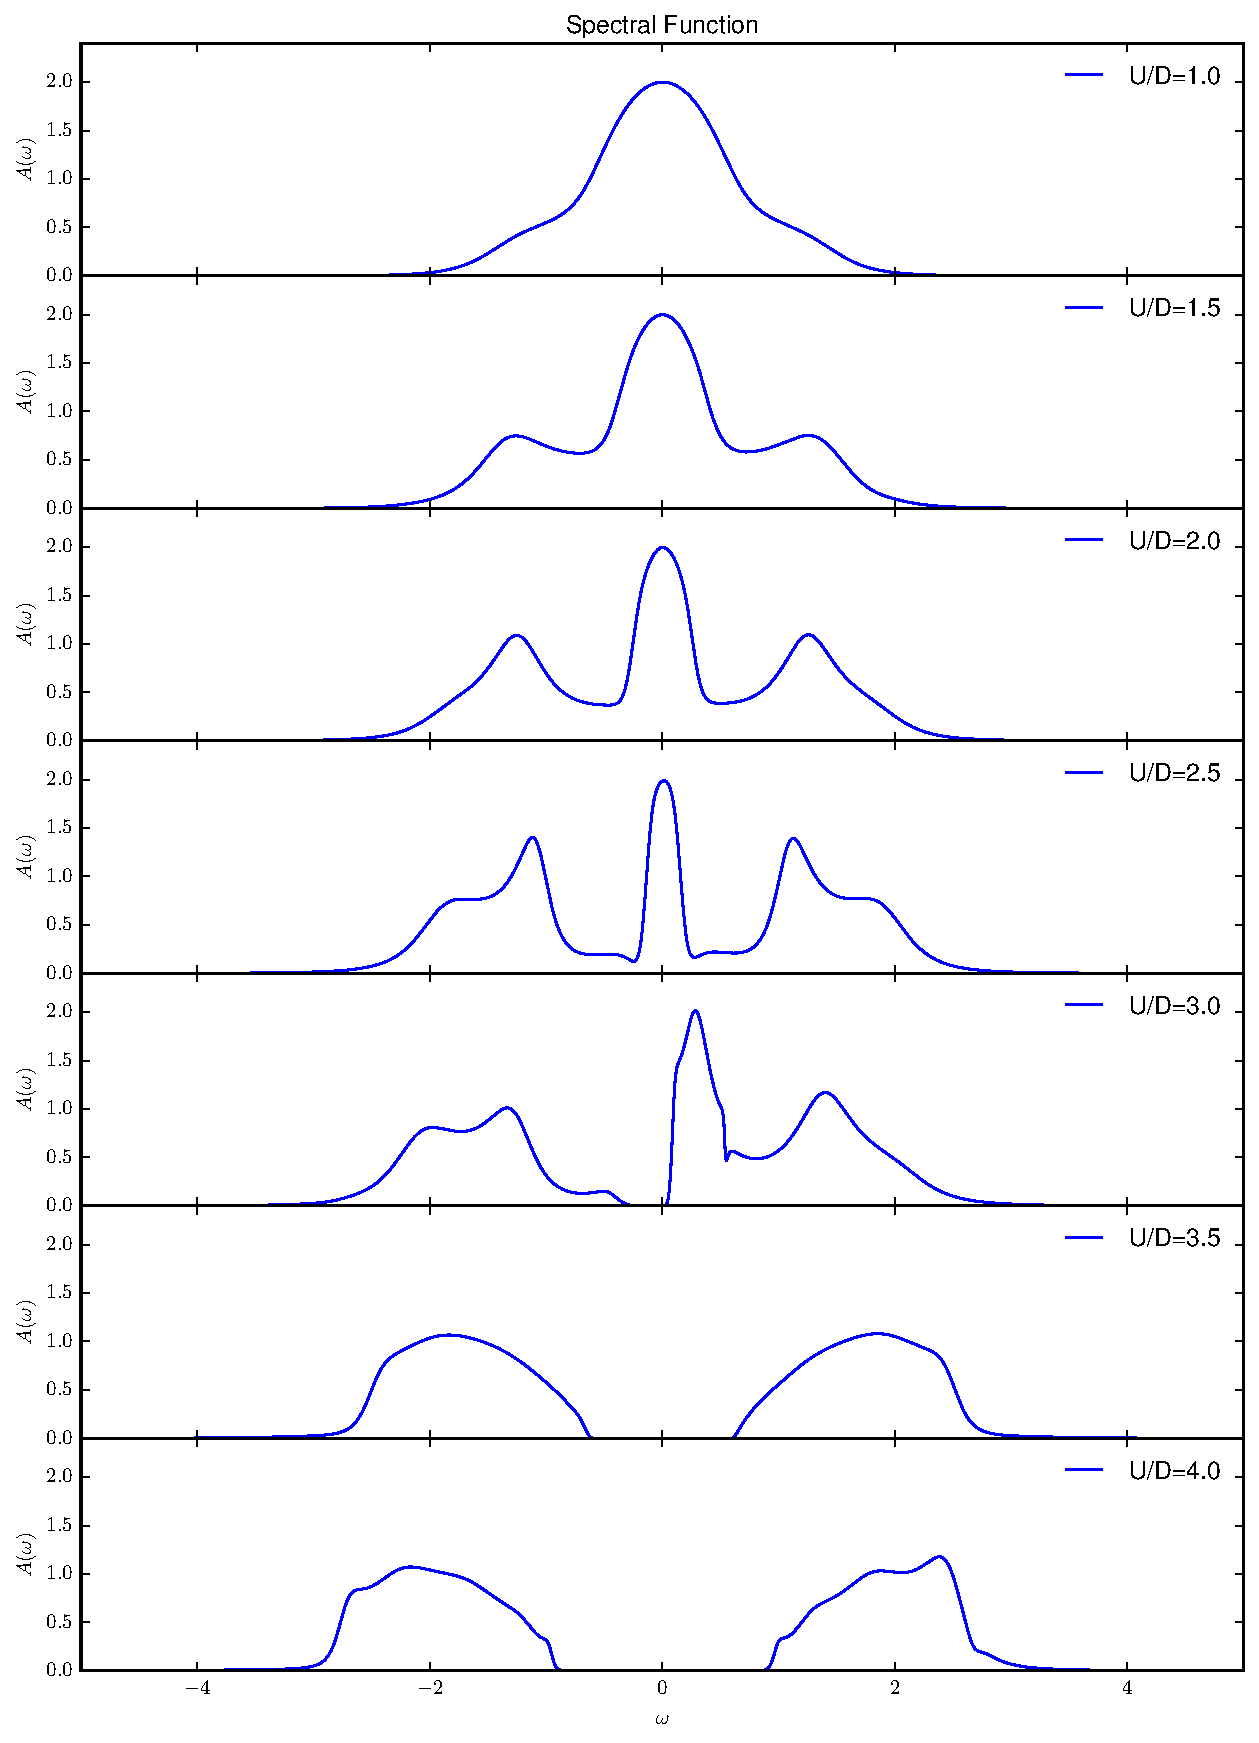
\includegraphics[width=0.5\textwidth ]{Mott_transition}
	\caption{Spectral function for varying parameters U. For low interaction parameter $U$ there are elementary excitation around zero frequency, which corresponds to the metallic phase. With increasing interaction parameter the spectral function develops a gap at zero freqency, hence the insulating phase.}
	\label{fig:spectralf}
\end{figure}
As a final result of our simulation, we obtained the plots of the Spectral~Function for increasing values of the interaction strenght $U$ (see \figref{fig:spectralf}).
It can cleary be seen that with increasing interaction we observe a phase transition (in our case between $3<U<4$) from a conductor to a Mott insulator, which is exactly what we expected to find. 

This deduction from the values of the spectral function at varying $U$ becomes clear if we recall the meaning of this function.  
In particular, for the Fermionic case, the single-particle Spectral~Function, $\mathcal{A(\bold{k},\omega)}$, can be expressed in the Lehmann representation: 

\begin{equation}\label{S.P.}
  \mathcal{A}(\omega) = \frac{1}{\mathcal{Z}}\sum_{n,m}|\braket{n|c_{\bold{\sigma},i}|m}|^2 (e^{-\beta E_n} + e^{-\beta E_m})\delta(\omega+(E_n-E_m))
\end{equation}
where the $\ket{n}$'s are the Hamiltonian eigenstates and the $E_n$'s are the corresponding energies. 
With the relations in \eqref{eq:Aprops} it is possible to interpret $A$ as a probability density. In particular, usually, this is interpreted as the probability of having a fermion with energy between $\omega$ and $\omega + \mathrm{d}\omega$.

In the light of this interpretation and of equation \eqref{S.P.}, it is clear that no gaps in the Spectral Function (as observed for low values of $U$) mean that we can produce excitations with any energy, leading to a conductive behavior. In contrast, if a gap is present (as for high values of $U$), no low-energy excitations, so that the material will behave as an insulator.


\clearpage
